\documentclass[11pt,a4paper]{article}
\usepackage[margin=1.2cm]{geometry}
\usepackage{amsmath,amssymb}
\usepackage{graphicx}
\usepackage{booktabs}
\usepackage{float}
\usepackage{array}
\usepackage{tabularx}
\usepackage[table]{xcolor}
\usepackage{enumitem}
\usepackage[hidelinks]{hyperref}
\usepackage{caption}
\usepackage{tikz}
\usetikzlibrary{positioning,fit,backgrounds,arrows.meta}
\usepackage{pgfplots}
\pgfplotsset{compat=1.17}
\usepgfplotslibrary{groupplots}

\captionsetup{font=small}
\setlist{nosep,leftmargin=1.3em}
\setlength{\parskip}{3pt}
\setlength{\parindent}{0pt}
\newcommand{\ci}[2]{[#1,\,#2]}
\newcommand{\term}[1]{\textbf{#1}}

\title{\textbf{Information Retrieval and Extraction --- Term Project}\\
       \large How Fast Does a News Recommender Go Stale, and How Often Must It Be Rebuilt?\\
       \normalsize Click-forward evaluation on EB-NeRD (main) and NPR (second dataset)}
\author{%
  Noel Alex Jacob (2025201085) \quad Emil Joji (2025201040) \\[1pt] Kspsvln Siddardha Kumar Kavuri (2025201061) \\[2pt]
  {\footnotesize \textit{CS4.406 Information Retrieval and Extraction -- IIITH -- Monsoon 2026}} \\[2pt]
  {\footnotesize \href{https://github.com/N03L-22/IRE_Proj_Draft}{\texttt{github.com/N03L-22/IRE\_Proj\_Draft}} (temporary share)}}
\date{}

\begin{document}
\maketitle
\setcounter{tocdepth}{1}
\tableofcontents
\vspace{-4pt}

% ============================================================
\section{The Question in One Page}
% ============================================================
A news recommender learns from what people clicked in the past. But news articles live for hours, not months. When the recommender is trained once and then left alone (we say it is \term{frozen}), the articles it learned about are soon gone and new ones arrive that it has never seen. We want to know three things:
\begin{enumerate}
\item \textbf{How fast} does a frozen recommender get worse?
\item \textbf{Which kind of signal} gets worse first: matching words, matching meaning, or learning from who clicked what?
\item \textbf{How often} must the recommender be rebuilt to stay good?
\end{enumerate}
The answer, in short (every number is explained later, with its confidence interval):
\begin{itemize}
\item \textbf{A recommender that learns from clicks goes stale within hours.} One hour after it is frozen it can still say something about 79\% of the clicks that follow. After 6 hours that is 19\%, after one day 0.9\%, and after three days none. New articles simply have no clicks yet.
\item \textbf{A recommender that reads the article text goes stale slowly, and only through the reader's profile.} If the reader's profile is frozen too, matching words loses about 10\% of its score in a week; if the profile is kept fresh, it loses almost nothing.
\item \textbf{Simply showing the newest articles first beats everything} on the main dataset, and never goes stale.
\item \textbf{How often to rebuild depends on the signal.} The click-based model needs a rebuild at least daily, and hourly on a busy news site. The text-based models can wait days, as long as the reader's profile stays current.
\end{itemize}

\begin{figure}[H]
\centering
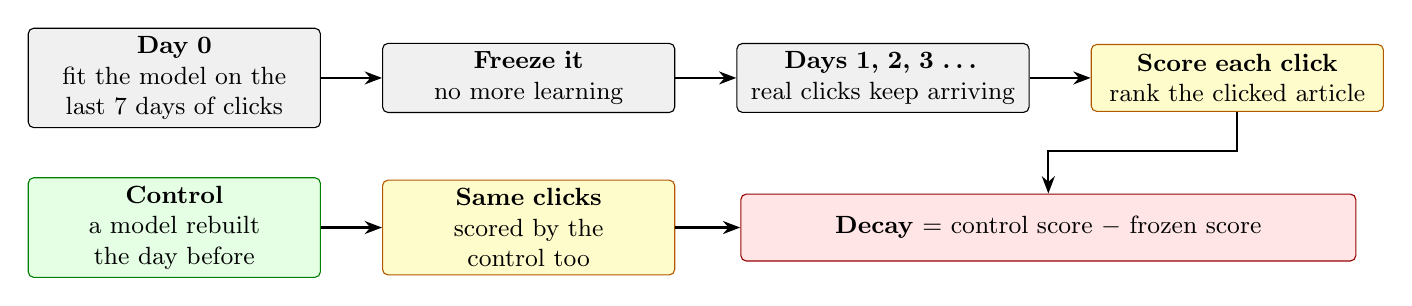
\begin{tikzpicture}[font=\small, node distance=0.9cm,
  box/.style={draw, rounded corners=2pt, fill=white, align=center, minimum height=0.85cm, text width=3.5cm, inner sep=3pt},
  arr/.style={-{Stealth[length=2.2mm]}, thick},
  region/.style={draw, rounded corners=4pt, thick, inner sep=8pt}]
  \node[box, fill=gray!12] (a) at (-6.2,0) {\textbf{Day 0}\\fit the model on the last 7 days of clicks};
  \node[box, fill=gray!12] (b) at (-1.7,0) {\textbf{Freeze it}\\no more learning};
  \node[box, fill=gray!12] (c) at (2.8,0) {\textbf{Days 1, 2, 3 \dots}\\real clicks keep arriving};
  \node[box, fill=yellow!20, draw=orange!70!black] (d) at (7.3,0) {\textbf{Score each click}\\rank the clicked article};
  \node[box, fill=green!10, draw=green!50!black] (e) at (-6.2,-1.9) {\textbf{Control}\\a model rebuilt the day before};
  \node[box, fill=yellow!20, draw=orange!70!black] (f) at (-1.7,-1.9) {\textbf{Same clicks}\\scored by the control too};
  \node[box, fill=red!10, draw=red!60!black, text width=7.6cm] (g) at (4.9,-1.9) {\textbf{Decay} = control score $-$ frozen score};
  \draw[arr] (a) -- (b); \draw[arr] (b) -- (c); \draw[arr] (c) -- (d);
  \draw[arr] (e) -- (f); \draw[arr] (f) -- (g); \draw[arr] (d.south) -- ++(0,-0.5) -| (g.north);
\end{tikzpicture}
\caption{The whole study in one picture. The same real clicks are scored by a frozen model and by a freshly rebuilt one; the difference is the decay.}
\end{figure}
\textit{Read it as:} the only thing that differs between the two scores is how old the model is.

% ============================================================
\section{Words We Use}
% ============================================================
\begin{center}
\small
\begin{tabularx}{\linewidth}{@{}lX@{}}
\toprule
\textbf{Word} & \textbf{Meaning}\\
\midrule
click & one reader opened one article at one moment\\
pool & the articles that could have been shown at the time of a click: published before it, in the last 48 hours\\
scorer & a method that gives every article in the pool a score; the highest score is shown first\\
fit date, frozen & the day the scorer learned from the past 7 days of clicks and then stopped learning\\
lag & days between the fit date and the click being scored\\
control & the same scorer, rebuilt the day before the click (lag 1)\\
\textbf{decay} & control score minus frozen score, on the same clicks; positive means the frozen model is worse\\
coverage & the share of clicked articles a frozen model is able to score at all\\
MRR & mean reciprocal rank: if the clicked article is ranked 1st it scores 1, 2nd gives $1/2$, 3rd gives $1/3$, and so on, averaged over clicks\\
top-10 hit rate & the share of clicks where the clicked article is among the first 10 (also called recall@10)\\
confidence interval & $[a,b]$ after a number: if we repeated the study on similar clicks, 95 out of 100 times the number would fall inside\\
\bottomrule
\end{tabularx}
\end{center}

% ============================================================
\section{The Scorers We Compare}
% ============================================================
We built the simplest scorers first and added complexity only to see what it buys.
\begin{center}
\small
\begin{tabularx}{\linewidth}{@{}lXX@{}}
\toprule
\textbf{Scorer} & \textbf{What it does} & \textbf{What it cannot do}\\
\midrule
Random shuffle & puts the pool in random order (the floor) & anything\\
Recency & newest article first & know what readers like\\
Popularity & most-clicked articles first & rank an article nobody has clicked yet\\
Word matching (BM25) & ranks articles by shared words with what the reader read before & see meaning (``car'' versus ``automobile'')\\
Meaning matching & a frozen multilingual MiniLM model turns each article into 384 numbers; articles close to what the reader read score high & use who else read what\\
Click history (co-click) & articles that the same people clicked together score high (cosine similarity) & score an article with no clicks or fewer than 5 readers\\
\bottomrule
\end{tabularx}
\end{center}
Two of these are the heart of the story. Word and meaning matching need only the \emph{text} of an article, which exists the moment it is published. Click history needs \emph{clicks}, which exist only after readers have found the article.

% ============================================================
\section{How We Measure It, Step by Step}
% ============================================================
\subsection{One click, one ranking}
Take one real click: reader $u$ opened article $a$ at time $t$. Build the pool (all articles published at or before $t$ and within the 48 hours before it). The scorer ranks the pool. We record the position of $a$.

\begin{table}[H]
\centering\small
\begin{tabular}{@{}rlr@{}}
\toprule
Rank & Article in the pool (invented toy example) & Score\\
\midrule
1 & Election results & 0.91\\
2 & Football transfer & 0.74\\
\rowcolor{green!15} 3 & \textbf{Storm warning (the clicked article)} & 0.66\\
4 & Cooking recipe & 0.30\\
5 & Celebrity gossip & 0.12\\
\bottomrule
\end{tabular}
\caption{A toy pool of five. The clicked article is 3rd, so the reciprocal rank is $1/3$, and it is inside the top 10. Real pools hold about 430 articles (EB-NeRD) or 1,500 (NPR).}
\end{table}
Averaged over thousands of clicks, this gives the MRR and the top-10 hit rate. Neither needs a person to say what was ``relevant'': the click itself is the truth, and it happens \emph{after} the model was frozen, so nothing leaks backwards.

\subsection{Freezing, waiting, comparing}
We fit every scorer on the 7 days of clicks ending on a \emph{fit date}, then score clicks on each later day. We use 14 fit dates (10--23 May 2023) and evaluation days 11--24 May, which gives 105 (fit date, day) cells. For each day the \term{control} is the model fitted the day before. \textbf{Decay = control $-$ frozen} on the same clicks. Each day has 20,000 clicks, chosen by a fixed-seed hash, out of 4--7 million.

\subsection{Two ways to treat the reader's profile}
Content scorers compare a candidate to what the reader read before. Which clicks count as ``before'' matters:
\begin{itemize}
\item \term{Frozen profile (regime A):} the clicks up to the fit date. The reader's recent reading is invisible.
\item \term{Live profile (regime B):} the last 50 clicks before the click. Only the article side is frozen.
\end{itemize}
Comparing A and B separates two kinds of staleness: the model's knowledge of articles and its knowledge of the reader.

\subsection{Rules that keep the numbers honest}
\begin{itemize}
\item \term{Already-read rule.} If the clicked article is already in the reader's own earlier clicks (15\% of clicks on EB-NeRD), it is a re-read, not a discovery; we leave it out and also remove the reader's history from every pool. This rule is the same for every scorer, so comparisons stay fair. (We first forgot it; see Section~\ref{sec:wrong}.)
\item \term{Cannot-score rule.} If a scorer cannot score an article, that article sits at the bottom, tied with the others in random order.
\item \term{Fresh versus decayed.} Each clicked article is placed into S0 (published before the fit ended), S1 (published after the fit but before the click day) or S2 (published on the click day). The three parts add up exactly to the decay, so we can say \emph{where} the loss comes from.
\item \term{Confidence intervals.} Every number is a mean with a 95\% bootstrap interval ($B=1000$). The frozen and control scores are resampled with the \emph{same} clicks (paired), which makes small differences visible.
\end{itemize}

% ============================================================
\section{The Data and the Pipeline}
% ============================================================
\begin{center}\small
\begin{tabular}{@{}lrrr@{}}
\toprule
 & \textbf{EB-NeRD} (main) & \textbf{NPR} (second) & \textbf{Adressa} (turnover only)\\
\midrule
Publisher, language & Ekstra Bladet, Danish & Globo, Portuguese & Norwegian news site\\
Days of clicks & 22 (May 2023) & 118 (Jan--Apr 2023) & 90 (Jan--Mar 2017)\\
Clicks, users & 113.4\,M, 791,582 & 17.6\,M, 1,162,802 & 35.2\,M, 3,614,911\\
Typical age of a clicked article & 1.4\,h & 13.8\,h & 5.8\,h\\
Evaluated here & 14 days $\times$ 20,000 clicks & 14 days, all impression clicks & no\\
\bottomrule
\end{tabular}
\end{center}
A \emph{typical clicked article is only 1.4 hours old} on EB-NeRD, against 13.8 hours on NPR. That one number predicts everything that follows. For EB-NeRD we use the click history of the validation users, because its volume and type of click are constant across dates. 27.2\% of the 4,468 articles published 4--25 May were never clicked.

\begin{figure}[H]
\centering
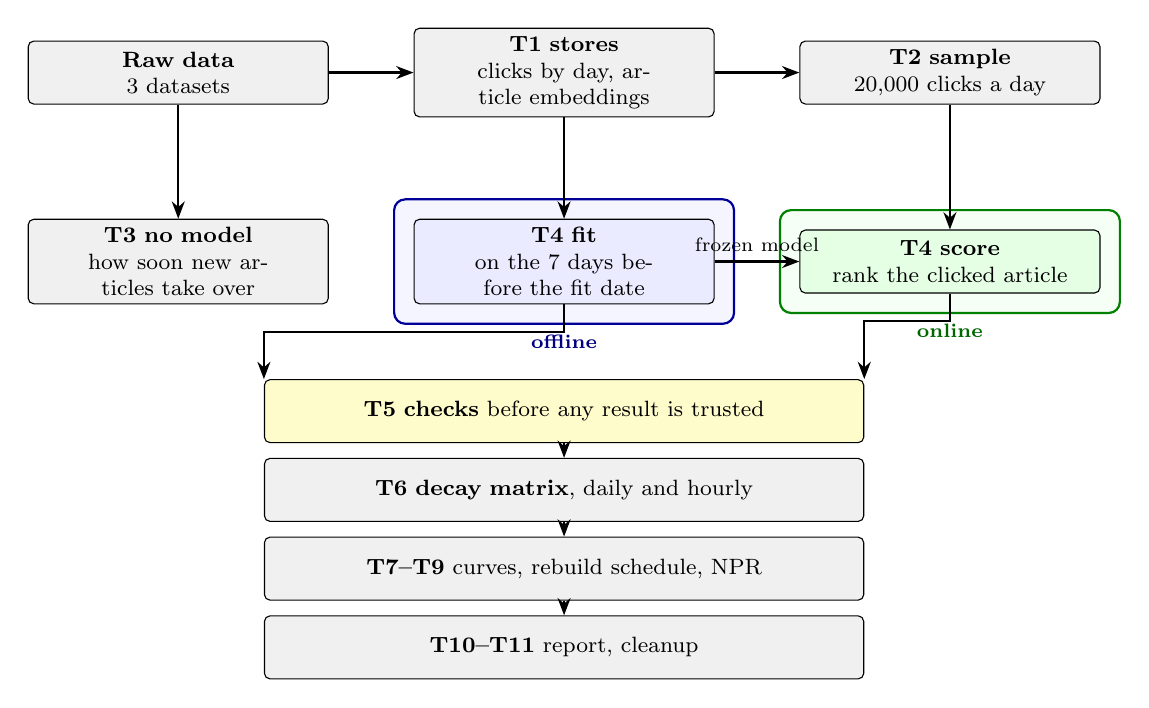
\begin{tikzpicture}[font=\footnotesize,
  box/.style={draw, rounded corners=2pt, fill=white, align=center, minimum height=0.8cm, text width=3.6cm, inner sep=3pt},
  wide/.style={box, text width=7.4cm},
  arr/.style={-{Stealth[length=2.2mm]}, thick},
  region/.style={draw, rounded corners=4pt, thick, inner sep=7pt}]
  \node[box, fill=gray!12] (raw) at (0,0) {\textbf{Raw data}\\3 datasets};
  \node[box, fill=gray!12] (store) at (4.9,0) {\textbf{T1 stores}\\clicks by day, article embeddings};
  \node[box, fill=gray!12] (samp) at (9.8,0) {\textbf{T2 sample}\\20,000 clicks a day};
  \node[box, fill=gray!12] (mf) at (0,-2.4) {\textbf{T3 no model}\\how soon new articles take over};
  \node[box, fill=blue!8] (fit) at (4.9,-2.4) {\textbf{T4 fit}\\on the 7 days before the fit date};
  \node[box, fill=green!10] (score) at (9.8,-2.4) {\textbf{T4 score}\\rank the clicked article};
  \node[wide, fill=yellow!20] (t5) at (4.9,-4.3) {\textbf{T5 checks} before any result is trusted};
  \node[wide, fill=gray!12] (mat) at (4.9,-5.3) {\textbf{T6 decay matrix}, daily and hourly};
  \node[wide, fill=gray!12] (an) at (4.9,-6.3) {\textbf{T7--T9} curves, rebuild schedule, NPR};
  \node[wide, fill=gray!12] (rep) at (4.9,-7.3) {\textbf{T10--T11} report, cleanup};
  \draw[arr] (raw) -- (store); \draw[arr] (store) -- (samp); \draw[arr] (store.south) -- (fit.north);
  \draw[arr] (samp.south) -- (score.north); \draw[arr] (raw.south) -- (mf.north);
  \draw[arr] (fit.east) -- node[above, font=\scriptsize]{frozen model} (score.west);
  \draw[arr] (fit.south) -- ++(0,-0.35) -| (t5.north west); \draw[arr] (score.south) -- ++(0,-0.35) -| (t5.north east);
  \draw[arr] (t5) -- (mat); \draw[arr] (mat) -- (an); \draw[arr] (an) -- (rep);
  \begin{scope}[on background layer]
    \node[region, draw=blue!60!black, fill=blue!4, fit=(fit), label={[blue!50!black, font=\scriptsize\bfseries]below:offline}] {};
    \node[region, draw=green!50!black, fill=green!4, fit=(score), label={[green!40!black, font=\scriptsize\bfseries]below:online}] {};
  \end{scope}
\end{tikzpicture}
\caption{The pipeline. Fitting (offline) and scoring (online) are kept apart, as in a real system. A monitor wraps every unit of work.}
\end{figure}

\textbf{Why you can trust the machinery.} Every unit of work writes its own file and a line with a hash in a manifest. The T5 gate checks that 1 worker, 2 workers, a reversed order and a resumed run give identical hashes; that recency has a decay of exactly 0 (its frozen and control models are the same function); that the three strata add up to the decay; that a pool allowed to contain post-click articles \emph{fails} (a mutation test); and two planted worlds. In a world with new articles arriving, the checks recover the planted click-history decay (0.0348 $\pm$ 0.0049); in a world with none, every decay is within 3.5 standard errors of zero (largest 1.87). 33 unit tests and 8 gate tests pass.

% ============================================================
\section{Results, One Step at a Time}
% ============================================================
\subsection{Step 1 --- How fast do new articles take over? (no model at all)}
Before any model: after a model is frozen, what share of the next clicks go to articles that were published \emph{after} the freeze? Such an article is unseen by any model fitted before it.
\begin{center}\small
\begin{tabular}{@{}lrrrrr@{}}
\toprule
 & 1 h & 3 h & 6 h & 12 h & 24 h\\
\midrule
EB-NeRD & 19.5 \ci{14.6}{23.9} & 77.2 \ci{72.7}{81.1} & \cellcolor{green!15}90.8 \ci{88.5}{92.5} & 95.4 \ci{94.8}{95.8} & 96.2 \ci{95.8}{96.5}\\
Adressa & 6.4 \ci{4.8}{8.3} & 24.8 \ci{21.6}{28.1} & \cellcolor{green!15}48.5 \ci{45.4}{51.5} & 73.2 \ci{71.3}{75.1} & 87.8 \ci{86.8}{88.7}\\
NPR & 1.0 \ci{0.7}{1.5} & 3.2 \ci{2.4}{4.2} & \cellcolor{green!15}15.5 \ci{11.3}{20.1} & 49.8 \ci{41.0}{58.2} & 85.6 \ci{80.6}{89.7}\\
\bottomrule
\end{tabular}
\end{center}
Percent of clicks that go to articles the frozen model never saw (13 fit days for EB-NeRD, 80 for Adressa, 85 for NPR; $n$ at 6 h: 3.46\,M, 1.26\,M, 72,136 clicks). \textit{Read it as:} on EB-NeRD, 6 hours after a freeze, nine clicks in ten go to something the model has never seen; on NPR it is fewer than two in ten. The hour of the fit matters too: a fit at midnight stays stale longer than one at 6 in the morning, because few articles are published overnight. EB-NeRD times are read as UTC, which is not confirmed.

\subsection{Step 2 --- A click-based model, hour by hour}
Now a real model. We froze every scorer at fits every 3 hours on 17--21 May and scored the next 24 hourly buckets of 5,000 clicks (40 cells per hour offset). Every hour is also the control of its own bucket. Regime A.

\begin{figure}[H]
\centering
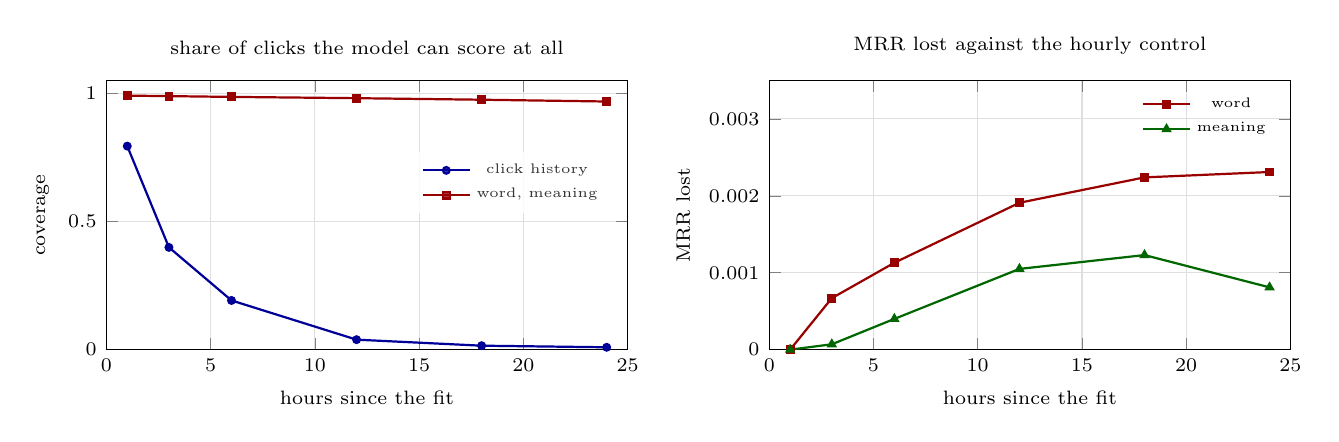
\begin{tikzpicture}
\begin{groupplot}[group style={group size=2 by 1, horizontal sep=1.8cm}, width=8.2cm, height=5.0cm, tick label style={font=\scriptsize}, label style={font=\scriptsize}, title style={font=\scriptsize}, legend style={font=\tiny, draw=none, fill=none}, xlabel={hours since the fit}, grid=major, grid style={gray!25}]
\nextgroupplot[title={share of clicks the model can score at all}, ylabel={coverage}, ymin=0, ymax=1.05, xmin=0, xmax=25, legend style={at={(0.97,0.62)}, anchor=east, font=\tiny, draw=none, fill=white, fill opacity=0.8}]
\addplot[blue!60!black, thick, mark=*, mark size=1.2pt] coordinates {(1,0.794)(3,0.399)(6,0.192)(12,0.039)(18,0.0155)(24,0.0093)};
\addlegendentry{click history}
\addplot[red!60!black, thick, mark=square*, mark size=1.2pt] coordinates {(1,0.991)(3,0.989)(6,0.986)(12,0.981)(18,0.975)(24,0.968)};
\addlegendentry{word, meaning}
\nextgroupplot[title={MRR lost against the hourly control}, ylabel={MRR lost}, ymin=0, ymax=0.0035, xmin=0, xmax=25, scaled y ticks=false, yticklabel style={/pgf/number format/fixed, /pgf/number format/precision=4}]
\addplot[red!60!black, thick, mark=square*, mark size=1.2pt] coordinates {(1,0)(3,0.00067)(6,0.00113)(12,0.00191)(18,0.00224)(24,0.00231)};
\addlegendentry{word}
\addplot[green!40!black, thick, mark=triangle*, mark size=1.4pt] coordinates {(1,0)(3,0.00007)(6,0.0004)(12,0.00105)(18,0.00123)(24,0.00081)};
\addlegendentry{meaning}
\end{groupplot}
\end{tikzpicture}
\caption{Hourly axis, EB-NeRD, regime A, 40 cells per point. Left: the click-history model collapses within hours. Right: the text models lose very little.}
\end{figure}
\begin{center}\scriptsize
\setlength{\tabcolsep}{3pt}
\begin{tabular}{@{}>{\raggedright\arraybackslash}p{3.8cm}rrrr@{}}
\toprule
 & 3 h & 6 h & 12 h & 24 h\\
\midrule
Click history coverage & 0.399 \ci{0.396}{0.401} & 0.192 \ci{0.191}{0.194} & 0.039 \ci{0.038}{0.040} & 0.0093 \ci{0.0088}{0.0097}\\
Word, MRR lost & 0.00067 \ci{0.00052}{0.00082} & 0.00113 \ci{0.00093}{0.00133} & 0.00191 \ci{0.00163}{0.00219} & 0.00231 \ci{0.00196}{0.00264}\\
Meaning, MRR lost & 0.00007 \ci{-0.00001}{0.00015} & 0.00040 \ci{0.00028}{0.00052} & 0.00105 \ci{0.00088}{0.00122} & 0.00081 \ci{0.00056}{0.00105}\\
\bottomrule
\end{tabular}
\end{center}
\textit{Read it as:} the click-based model loses almost all of its reach in a day; the text models lose a few thousandths of an MRR point. Word matching's 24-hour loss, 0.0023 of its 0.0322, is 7\%. On the clicks the click-history model can still score at 6 h its top-10 hit rate is 0.045 against 0.104 for the control (a loss of 0.059 \ci{0.055}{0.062}); at 24 h only 0.9\% of clicks are scorable and the loss is undetermined (0.009 \ci{-0.009}{0.028}).

\subsection{Step 3 --- Days, not hours: the profile is what ages}
The daily matrix has 14 fit dates and lags of 1 to 13 days. Clicks scored: 236,387 at lag 1, 202,331 at lag 3, 135,583 at lag 7 and 34,479 at lag 13 (there are fewer pairs at long lags; lag 13 is a single cell).
\begin{center}\scriptsize
\setlength{\tabcolsep}{3pt}
\begin{tabular}{@{}llrrrr@{}}
\toprule
 & & lag 1 & lag 3 & lag 7 & lag 13\\
\midrule
Word, frozen profile (A) & MRR & 0.0310 \ci{0.0306}{0.0314} & 0.0309 \ci{0.0305}{0.0313} & 0.0299 \ci{0.0295}{0.0305} & 0.0248 \ci{0.0239}{0.0258}\\
\rowcolor{green!12} & \textbf{lost} & 0 & 0.0008 \ci{0.0004}{0.0012} & \textbf{0.0030} \ci{0.0024}{0.0036} & \textbf{0.0059} \ci{0.0047}{0.0071}\\
Word, live profile (B) & MRR & 0.0325 \ci{0.0321}{0.0329} & 0.0331 & 0.0341 \ci{0.0336}{0.0347} & 0.0313\\
 & lost & 0 & -- & 0.00013 \ci{0.00007}{0.00019} & --\\
Meaning, frozen (A) & MRR & 0.0250 \ci{0.0247}{0.0253} & 0.0247 & 0.0240 \ci{0.0236}{0.0244} & 0.0212 \ci{0.0204}{0.0221}\\
 & lost & 0 & -0.0002 \ci{-0.0004}{0.0001} & 0.0007 \ci{0.0003}{0.0011} & 0.0013 \ci{0.0005}{0.0022}\\
Meaning, live (B) & MRR, lost & 0.0259, 0 & 0.0253, 0 & 0.0253, 0 & 0.0233, 0\\
Random shuffle & MRR & 0.0172 & 0.0177 & 0.0176 & 0.0150\\
Recency & MRR & 0.190 & 0.195 & 0.196 & 0.179\\
\bottomrule
\end{tabular}
\end{center}
\begin{figure}[H]
\centering
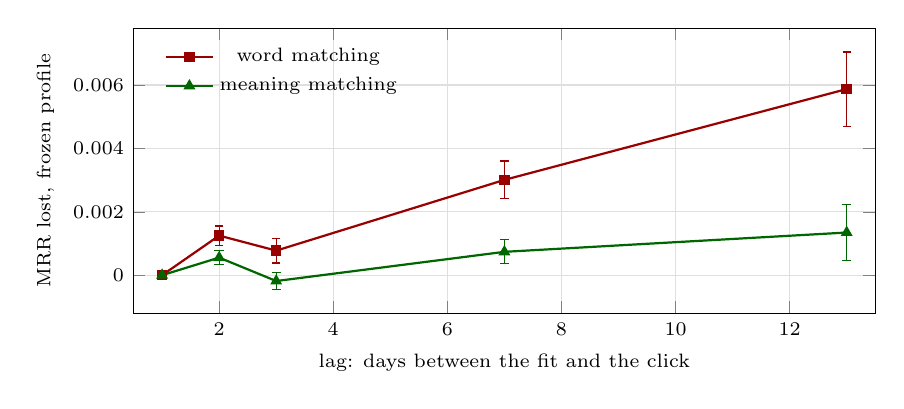
\begin{tikzpicture}
\begin{axis}[width=11cm, height=5.2cm, xlabel={lag: days between the fit and the click}, ylabel={MRR lost, frozen profile}, tick label style={font=\scriptsize}, label style={font=\scriptsize}, legend style={font=\scriptsize, at={(0.03,0.97)}, anchor=north west, draw=none, fill=none}, grid=major, grid style={gray!25}, xmin=0.5, xmax=13.5, scaled y ticks=false, yticklabel style={/pgf/number format/fixed, /pgf/number format/precision=4}]
\addplot[red!60!black, thick, mark=square*, mark size=1.5pt, error bars/.cd, y dir=both, y explicit] coordinates {(1,0) +- (0,0) (2,0.001249) +- (0,0.000303) (3,0.000775) +- (0,0.000389) (7,0.003006) +- (0,0.000597) (13,0.005871) +- (0,0.001170)};
\addlegendentry{word matching}
\addplot[green!40!black, thick, mark=triangle*, mark size=1.7pt, error bars/.cd, y dir=both, y explicit] coordinates {(1,0) +- (0,0) (2,0.000555) +- (0,0.000218) (3,-0.000184) +- (0,0.000264) (7,0.000737) +- (0,0.000377) (13,0.001346) +- (0,0.000889)};
\addlegendentry{meaning matching}
\end{axis}
\end{tikzpicture}
\caption{Daily decay of the text scorers with a frozen profile. Bars are the 95\% intervals. The loss grows steadily with lag.}
\end{figure}
\textit{Read it as:} with a frozen profile, word matching is about 10\% worse after a week and 24\% worse after nearly two. With a live profile the loss vanishes. Meaning matching with a live profile loses exactly 0, because its article vectors do not depend on the fit and the profile is rebuilt from clicks, so the frozen and control models are the same function. \textbf{So the text signal goes stale because the reader's recent interests are missing, not because the articles are old.} Both text scorers are weak (2 to 3 times the shuffle); recency is far ahead (top-10 hit rate 0.515 \ci{0.513}{0.517} against 0.061 for word matching and 0.027 for the shuffle).

\textbf{Click history and popularity, day by day.} Their overall MRR looks \emph{worse than the shuffle} (0.0079 \ci{0.0077}{0.0080} for click history at lag 1 against 0.0172), which would be a misleading way to read it. A target they cannot score is placed below older articles they \emph{can} score, so ``cold-start'' clicks are penalised. The honest measure is coverage: 12.0\% at lag 1, 0.4\% at lag 2, zero from lag 3 (the hourly curve above is the same story at finer resolution). On the clicks they \emph{can} score, accuracy is fine; for click history at lag 2 it is 0.139 against 0.141 for the control (0.002 \ci{-0.015}{0.020}), but that is 0.4\% of clicks.

\subsection{Step 4 --- Where does the loss sit?}
For word matching with a live profile at lag 7, the total loss is 0.00013. Almost all of it comes from articles published on the click day itself (S2: 0.00012); articles published after the fit but before the day (S1) contribute 0.000006. So the text models lose accuracy on the \emph{newest} articles, not on old ones. For click history at lag 3 the S2 term is $-0.0117$ and the S1 term $+0.0024$; their sum is what the cold-start rule produces, which is why coverage is the better measure for this scorer.

\subsection{Step 5 --- How often should it be rebuilt?}
We replayed the same cells with a rebuild every $k$ days, so day $d$ uses the latest rebuild at or before $d-1$. MRR over 14 days, with the cost of the fits:
\begin{center}\small
\begin{tabular}{@{}lrrr@{}}
\toprule
Rebuild every & 1 day (14 fits) & 7 days (2 fits) & 14 days (1 fit)\\
\midrule
Word, frozen profile (A) & \cellcolor{green!12}0.0310 \ci{0.0306}{0.0314} & 0.0298 \ci{0.0295}{0.0302} & 0.0274 \ci{0.0270}{0.0277}\\
Word, live profile (B) & 0.0325 \ci{0.0321}{0.0329} & 0.0324 \ci{0.0320}{0.0328} & 0.0324 \ci{0.0320}{0.0327}\\
Meaning, A and B & \multicolumn{3}{c}{identical at every interval}\\
Click history (B) & 0.0079 \ci{0.0077}{0.0080} & 0.0148 \ci{0.0146}{0.0151} & 0.0161 \ci{0.0158}{0.0163}\\
Total fit time & 306 s (click history), 29 s (word) & 44 s, 4 s & 22 s, 2 s\\
\bottomrule
\end{tabular}
\end{center}
\textit{Read it as:} with a frozen profile, daily rebuilding of word matching gains 12\% over a single rebuild; with a live profile it gains nothing. The apparent rise of click history with a longer interval is a coverage artefact: an older, wider window reaches more of the older articles in the pool, and fewer targets are cold. It is \emph{not} evidence that a stale click-history model is better. One click-history fit costs about 22 s and a peak near 7\,GB. A hybrid that falls back to recency for unscorable articles was not built, so these intervals apply to each signal alone.

\subsection{Step 6 --- A second site: NPR}
NPR (Portuguese, a slower news cycle) has 14 fit and evaluation days (10--24 March 2023), all impression clicks, 119,172 at lag 1. The pool is about 1,500 articles. Regime A, lag 1, MRR: popularity 0.162 \ci{0.161}{0.163}, click history 0.105 \ci{0.104}{0.107}, word 0.0181 \ci{0.0175}{0.0187}, meaning 0.0179 \ci{0.0174}{0.0185}, recency 0.0066 \ci{0.0065}{0.0068}, shuffle 0.0058 \ci{0.0056}{0.0060}. Top-10 hit rate: popularity 0.550 \ci{0.547}{0.553}, click history 0.249 \ci{0.246}{0.251}.
\begin{itemize}
\item \textbf{The ranking of signals is different.} Here popularity and click history are best and recency is no better than the shuffle, because articles live longer (typical age 13.8 h) and the pool is 1,500 articles. A lesson: \emph{which signal to rebuild how often depends on the site}.
\item Coverage stays high for click history (97\% at lag 1, 96\% at lag 7) because new articles take over slowly (only 15.5\% unseen at 6 h).
\item Word matching with a frozen profile loses 0.0012 \ci{0.0010}{0.0015} at lag 3 and 0.0024 \ci{0.0020}{0.0029} at lag 7 (14\% of its 0.0167); meaning loses 0.0022 \ci{0.0017}{0.0027} at lag 7. The text-model story repeats.
\item \textbf{Unexplained.} Popularity gets \emph{better} with an older fit (its ``decay'' at lag 3 is $-0.112$ \ci{-0.113}{-0.111} MRR). We have not found the cause and report it only as a measurement.
\end{itemize}

\subsection{Step 7 --- Checks on our own results}
\textbf{Does removing never-clicked articles change the story?} 27.2\% of the articles in the pool were never clicked in the whole corpus. A recommender cannot know that in advance (it uses future clicks), so this is an oracle ceiling, not a realistic setting. We removed them from every pool, with identical clicks (17,037 on the first fit in both runs). Regime B, lag 1, top-10 hit rate:
\begin{center}\small
\begin{tabular}{@{}lrrr@{}}
\toprule
 & Recency & Shuffle & Meaning / Word\\
\midrule
All articles in the pool & 0.515 \ci{0.513}{0.517} & 0.027 \ci{0.026}{0.027} & 0.047 / 0.061\\
Never-clicked removed & 0.634 \ci{0.632}{0.636} & 0.040 \ci{0.039}{0.041} & 0.062 \ci{0.061}{0.063} / 0.063 \ci{0.062}{0.064}\\
\bottomrule
\end{tabular}
\end{center}
Every level rises, but the decay does not change: word matching, live profile, MRR lost at lag 7 is 0.00013 in the main run and 0.00010 \ci{0.00003}{0.00016} here; meaning and recency stay at 0. \textit{So the pool noise lifts every score equally and the staleness result stands.}

\textbf{Does decay follow the amount of news per day? (exploratory)} At lag 3 over 12 days, Spearman $\rho$ between word MRR lost and articles published that day (152--266) is $-0.42$ \ci{-0.87}{0.24}; against clicks that day (4.2--6.8\,M) $-0.52$ \ci{-0.98}{0.20}. For click history $+0.43$ \ci{-0.14}{0.81} and $-0.20$ \ci{-0.77}{0.55}. Every interval includes 0: \textbf{no relation is detectable} with 12 days from one site. This needs a longer span or more sites.

% ============================================================
\section{The Answer, Put Together}
% ============================================================
\begin{center}\small
\begin{tabularx}{\linewidth}{@{}lXX@{}}
\toprule
\textbf{Signal} & \textbf{Why it goes stale} & \textbf{How often to rebuild (EB-NeRD)}\\
\midrule
Recency & it does not & never\\
\rowcolor{green!12} Click history & new articles have no clicks: coverage 79\% at 1 h, 19\% at 6 h, 0.9\% at 24 h & at least daily; hourly on a busy site (one fit: 22 s, about 7\,GB)\\
Popularity & the same, because it counts clicks & the same as click history\\
Word matching & the reader's profile ages (10\% lost in 7 days, 24\% in 13); articles hardly matter & keep the profile live; the word index itself can wait about a week\\
Meaning matching & only a small profile effect (0.0007 \ci{0.0003}{0.0011} by lag 7); article vectors never change & never for decay; refresh the profile\\
\bottomrule
\end{tabularx}
\end{center}
\textbf{Why the same models decay differently on another site.} What predicts the decay is how quickly articles take over (Section 6.1): 91\% unseen at 6 h on EB-NeRD, 49\% on Adressa, 16\% on NPR. A site with slower turnover can rebuild less often.

% ============================================================
\section{What Went Wrong, and What We Changed}\label{sec:wrong}
% ============================================================
\begin{itemize}
\item \textbf{We scored articles the reader had already read (the main error).} Our first full run included re-reads. Our own check found that 15\% of the clicked articles were already in the reader's history, and that already-read articles outranked the target. This inflated word matching (MRR 0.0573 with them, 0.0143 without) and made a fresher profile look worse. We deleted every result of that run and reran everything under the already-read rule.
\item \textbf{Two hourly units were marked complete but 19 of their files were missing.} Found when the analysis failed; recomputed. The cause is unknown. A manifest-versus-files check belongs in the final cleanup.
\item \textbf{We said word matching ``barely goes stale''.} That was true only for the live profile. With a frozen profile it loses 10\% in a week (Step 3). Corrected here and in the mid-submission report.
\item \textbf{Memory.} Click history needs about 7\,GB per fit, not the 1.5\,GB we planned, so only two workers run at once.
\item \textbf{The corpus.} Our first plan assumed one uniform click corpus. EB-NeRD is not uniform, so we chose click-forward evaluation on one cohort.
\item \textbf{Duplicate rows} in the first stores (107,633 in NPR, 7,693 in Adressa), found by counting and rebuilt.
\end{itemize}
The full record (decisions D1--D28, findings P1--P48, dated errata, session log) is in \texttt{log.md}.

% ============================================================
\section{Limits, Stated Plainly}
% ============================================================
\begin{itemize}
\item \textbf{One main site, one month, one cohort} (the validation users), 14 fit days. NPR is a second site; Adressa has the turnover measure only.
\item \textbf{The negatives are the other pool articles}, not real impression slates, so levels are low and overall MRR is penalised by cold start. We report coverage next to it. The team still has to pick the headline metric.
\item \textbf{The 48-hour pool window, the sample size and the seed were not varied.} Sensitivity runs were planned and not done.
\item \textbf{EB-NeRD times are assumed to be UTC.} Hour labels may be shifted by 1--2 hours.
\item \textbf{Decay is measured against a model rebuilt one day (or one hour) earlier.} Faster rebuilds were not tested. The bootstrap treats days as given, so intervals do not cover day-to-day variation.
\item \textbf{No hybrid model} (recency as a fallback for unscorable articles) and no position-based baseline were built.
\item \textbf{Popularity improving with an older fit on NPR is unexplained.}
\item \textbf{The never-clicked check and the volume check are not realistic settings or findings}; they are labelled as such.
\end{itemize}

% ============================================================
\section{Reproducing This Report}
% ============================================================
\raggedright From \texttt{code/}, with the project's Python environment (\texttt{<root>} is the project folder):
\begin{itemize}
\item \textbf{Daily matrix:} \texttt{decay.py <root> --fits 2023-05-10 2023-05-23 --last 2023-05-24}
\item \textbf{Hourly:} \texttt{decayh.py <root> --first 2023-05-17 --last 2023-05-22 --fit-days 2023-05-17 2023-05-21 --step 3}
\item \textbf{Tables with intervals:} \texttt{analyze.py <root>} and \texttt{analyze\_hourly.py <root>}
\item \textbf{NPR:} the same with \texttt{--name npr --out results/npr/decay\_matrix}
\item \textbf{Never-clicked check:} \texttt{decay.py} with \texttt{--clicked-only --out results/sens\_clicked\_only/decay\_matrix}
\item \textbf{Volume check and gate:} \texttt{volume\_check.py <root>}, \texttt{test\_t5.py}
\end{itemize}
Data stays under \texttt{data/} (not in the repository). Run logs and the gate record are in \texttt{results/metrics/}. The Adressa tarball was never extracted.

\end{document}
